\documentclass[11pt]{beamer}
\usetheme{Frankfurt}
\usecolortheme{crane}
\usepackage[utf8]{inputenc}
\usepackage[english]{babel}
\usepackage{amsmath}
\usepackage{amsfonts}
\usepackage{amssymb}
\usepackage{graphicx}
%\usepackage{circuitikz}
\author{Maximilian Heim}
\title{Hardware Trojan Detection}
%\setbeamercovered{transparent} 
%\setbeamertemplate{navigation symbols}{} 
\logo{
\includegraphics[width=1.5cm]{1200px-Hsas_logo.svg.png}}
\institute{University Albstadt-Sigmaringen} 
\date{\today} 
\subject{Hardware Cyber-Security}
\begin{document}

\begin{frame}
\titlepage
\end{frame}

\begin{frame}
\tableofcontents
\end{frame}

\section{Introduction}
\subsection{Hardware Trojans}
\begin{frame}
    \frametitle{Was sind Hardware Trojaner?}
    \begin{enumerate}
    \item Bösartige Modifikation eines Integrierten Schaltkreises
    \item Besteht aus einem Trigger (Time bombs, cominational...) und einer Payload (Denial of service, extraction of information, keys)
    \end{enumerate}
    \begin{figure}
        \caption{Theoretischer Aufbau eines HW Trojaners}
        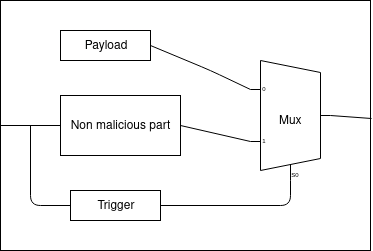
\includegraphics[width=0.5\textwidth]{triggerpayload.png}
        \label{trpl}
    \end{figure}
\end{frame}

\subsection{Relevanz}
\begin{frame}
    \frametitle{Warum ist es wichtig diese zu erkennen?}
    \begin{itemize}
    \item Militär
    \item Finanzen
    \item Energie
    \item Geheimdienste
    \item Überwachungsstaaten
    \item Transport
    \item U.v.m \ldots
    \end{itemize}
\end{frame}


\section{Erkennung}
\subsection{Destruktive Erkennung}
\begin{frame}
    \frametitle{Reverse Engineering}
    \begin{itemize}
        \item Entfernen der Oberfläche Schicht für Schicht, vergleich mit Golden Sample
        \item Vorteile: 
        \begin{enumerate}
            \item 100 \% Erkennungsrate mit passendem Equipment
        \end{enumerate}
        \item Nachteile:
        \begin{enumerate}
            \item Testet nur einen Chip
            \item Chip ist danach kaputt
            \item Sehr zeitaufwändig
        \end{enumerate}
    \end{itemize}
\end{frame}
\subsection{Nicht-Destruktive Erkennung}
\begin{frame}
    \frametitle{Funktionstests}
    \begin{itemize}
        \item Beobachten der Ausgabe bei bestimmten Eingängen und Vergleich dieser mit Golden Sample
        \item Problem: Trigger sehr spezifisch, daher wird hier zum Teil auch mit Fuzzing gearbeitet
        \item Vorteile:
        \begin{enumerate}
            \item Sehr einfacher Testaufbau
            \item Hohe Erkennungsrate
            \item Hunderte IC's können parallel getestet werden
        \end{enumerate}
        \item Nachteile:
        \begin{enumerate}
            \item Je nach Komplexität des IC's sehr zeitaufwändig/unmöglich
        \end{enumerate}
    \end{itemize}
\end{frame}

\begin{frame}
    \frametitle{Seitenkanaltest}
    \begin{itemize}
        \item Beobachten der Leistungsaufnahme/Pfadverzögerung des IC's und Vergleich dieser mit dessen eines Golden Samples
        \item Vorteile:
        \begin{enumerate}
            \item Erkennung ohne Aktivierung
            \item Sehr einfacher Testaufbau
            \item Hohe Erkennungsrate
            \item Hunderte IC's können parallel getestet werden
        \end{enumerate}
        \item Nachteile:
        \begin{enumerate}
            \item Produktionsvariationen
            \item Bei sehr kleinen Trojanern kann die Leakage sehr klein werden
        \end{enumerate}
        \item D. Agrawal und andere stellen in “Trojan detection using IC fingerprinting” das Konzept von IC Fingerprinting vor. Hier wird basierend auf einem oder mehreren Seitenkanälen ein Fingerabdruck erzeugt der Trojaner mit einem Flächeanteil von 0.01 \% erkennt.
    \end{itemize}
\end{frame}

\section{Fazit}
\begin{frame}
    \frametitle{Fazit}
\end{frame}

\begin{frame}
    \frametitle{Quellen}
    \begin{itemize}
    \item \url{https:/d/dl.acm.org/doi/pdf/10.1145/2906147}
    \item \url{https://ieeexplore.ieee.org/stamp/stamp.jsp?tp=&arnumber=5340158}
    \end{itemize}
\end{frame}

\end{document}